\chapter{الهيدروجين وعناصر الفئة s}\label{ch:b1:s-block}

كل هاتف وحاسوب محمول وسيارة كهربائية يحمل بطارية تحمل شحناتِها
الموجبةَ أيوناتُ الليثيوم. ويأتي ذلك الليثيوم أساسًا من مكانين:
مناجم الصخور الصلبة في أستراليا والسبخات الملحية في جبال الأنديز، حيث
يُضخ المحلول الملحي من تحت القشرة ويُترك ليتبخر تحت الشمس طوال
أشهر حتى يمكن ترسيب أملاح الليثيوم منه. والليثيوم هو
أول \omterm{def:b1:s-block:families}{الفلزات القلوية}، وهي أنشط الفلزات على الإطلاق، وجيرانه
الصوديوم والبوتاسيوم والمغنيزيوم والكالسيوم يوفّرون المواد الكيميائية الأساسية
للصناعة: الصودا الكاوية، ورماد الصودا، والجير. يفتح هذا الفصل
الكيمياء الوصفية للعناصر بالهيدروجين وعناصر \omterm{def:b1:periodicity:table}{الفئة} s،
مستعملًا أدوات الفصول السابقة --- طاقات التأين،
\omterm{def:b1:nernst:electrode-potential}{والجهود المعيارية}، \omterm{def:b1:precipitation:solubility-product}{وجداءات الذوبانية} --- لتفسير سلوك هذه
العناصر.

\begin{recall}
طاقات التأين \omterm{def:b1:periodicity:electronegativity}{والكهرسلبية} (\cref{ch:b1:periodicity})؛
\omterm{def:b1:nernst:electrode-potential}{والجهود المعيارية} (\cref{ch:b1:nernst})؛ \omterm{def:b1:precipitation:solubility-product}{وجداءات الذوبانية}
وترسيب الهيدروكسيدات (\cref{ch:b1:precipitation}). وقد صنّف المجلد
المدرسي (الصف العاشر) العناصر في عائلات: \omterm{def:b1:s-block:families}{الفلزات القلوية}،
\omterm{def:b1:s-block:families}{والفلزات القلوية الترابية}، والهالوجينات، والغازات النبيلة.
\end{recall}

\begin{omfigure}
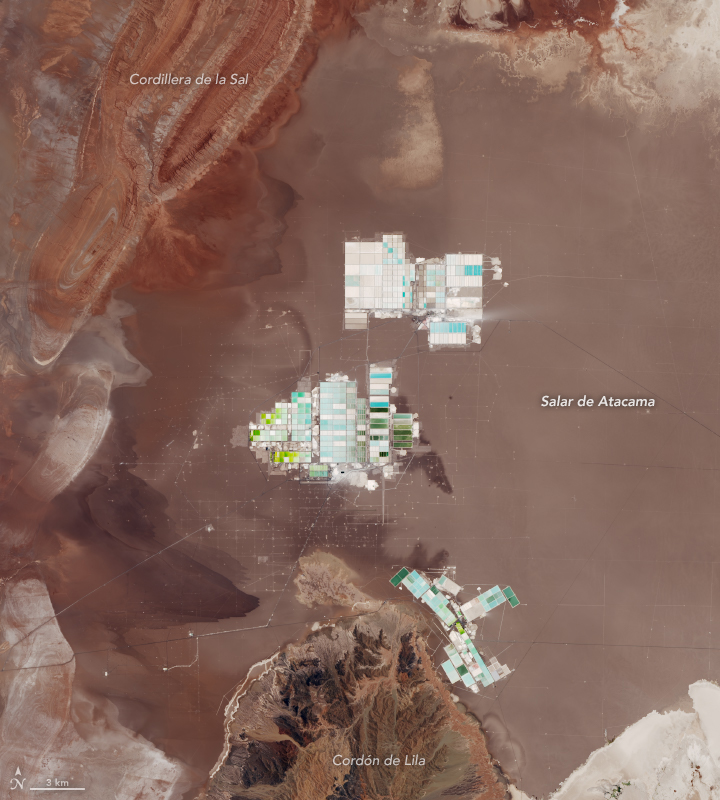
\includegraphics[width=0.48\linewidth]{images/book2/atacama-ponds.jpg}

{\small أحواض تبخير المحلول الملحي الليثيومي في سبخة أتاكاما، كما تُرى
من المدار (لاندسات 8، 2018؛ مرصد الأرض التابع لناسا، ملكية عامة،
ويكيميديا كومنز). ويتغيّر لون كل حوض كلما
تركّز المحلول الملحي وتبلورت الأملاح.}
\end{omfigure}

\section{الهيدروجين والهيدريدات}

للهيدروجين إلكترون واحد: فيمكنه أن يفقده (\ce{H+}، الذي يحمله الماء على هيئة
\ce{H3O+})، أو أن يشارك به (\omterm{def:b1:lewis-resonance-vsepr:lewis}{روابط تساهمية})، أو أن يكتسب إلكترونًا (\ce{H-}، \omterm{def:b1:quantum-numbers:configuration}{بالتوزيع
الإلكتروني} للهيليوم). وأيّها يفعل يتعلق بشريكه.

\begin{definition}[الهيدريدات]\label{def:b1:s-block:hydride}
\emph{الهيدريد}\index{هيدريد} مركب ثنائي للهيدروجين مع
عنصر آخر. و\emph{الهيدريدات الملحية}\index{هيدريد ملحي}، المتكوّنة
مع \omterm{def:b1:s-block:families}{الفلزات القلوية} \omterm{def:b1:s-block:families}{والفلزات القلوية الترابية} الأثقل (\ce{LiH}، \ce{NaH}،
\ce{CaH2})، أجسام صلبة أيونية تحتوي \ce{H-}. و\emph{الهيدريدات
التساهمية}\index{هيدريد تساهمي}، المتكوّنة مع عناصر \omterm{def:b1:periodicity:table}{الفئة} p
(\ce{CH4}، \ce{NH3}، \ce{H2O}، \ce{HCl})، جزيئية. و\emph{الهيدريدات
الفلزية}\index{هيدريد فلزي}، المتكوّنة مع بعض الفلزات الانتقالية،
أجسام صلبة يشغل فيها الهيدروجين \omterm{def:b1:crystals-metals:site}{المواقع البينية} في \omterm{def:b1:crystals-metals:lattice}{الشبكة}
الفلزية، وكثيرًا ما يكون تركيبها متغيرًا.
\end{definition}

أيون \omterm{def:b1:s-block:hydride}{الهيدريد} قاعدة \omterm{def:b1:nernst:couple}{ومختزل} قويان جدًا: \omterm{def:b1:s-block:hydride}{فالهيدريدات الملحية}
تتفاعل مع الماء، \ce{NaH + H2O -> NaOH + H2}، وتُستعمل عوامل تجفيف
للمذيبات وقواعد في التخليق العضوي (\cref{ch:b1:alcohol-activation}).
وتُظهر \omterm{def:b1:s-block:hydride}{الهيدريدات التساهمية} لعناصر \omterm{def:b1:periodicity:table}{الدورة} الثانية منحى
\omterm{def:b1:periodicity:electronegativity}{الكهرسلبية} على امتدادها: \ce{CH4} ليس حمضيًا ولا قاعديًا، و\ce{NH3}
قاعدي، و\ce{H2O} مذبذب، و\ce{HF} حمضي.

\section{الفلزات القلوية}

\begin{definition}[الفلزات القلوية والفلزات القلوية الترابية]\label{def:b1:s-block:families}
\emph{الفلزات القلوية}\index{فلز قلوي} (Li، Na، K، Rb، Cs، Fr) تكوّن
\omterm{def:b1:periodicity:table}{الزمرة} 1، ولها \omterm{def:b1:quantum-numbers:configuration}{إلكترون تكافؤ} واحد \babelsublr{\textit{ns}$^1$}؛
و\emph{الفلزات القلوية الترابية}\index{فلز قلوي ترابي} (Be، Mg، Ca، Sr،
Ba، Ra) تكوّن \omterm{def:b1:periodicity:table}{الزمرة} 2، ولها \babelsublr{\textit{ns}$^2$}. وعناصرها هي
\omterm{def:b1:periodicity:table}{الفئة} s.
\end{definition}

\begin{proposition}[الفلزات القلوية مختزلات قوية]\label{prop:b1:s-block:reducing-power}
للفلزات القلوية أدنى طاقات تأين أولى في
دوراتها (Li \qty{5.39}{eV}، Na 5.14، K 4.34) \omterm{def:b1:nernst:electrode-potential}{وجهود معيارية} سالبة
جدًا ($\ce{Li+}/\ce{Li}$ \babelsublr{$-3.04$~V}، $\ce{Na+}/\ce{Na}$ $-2.71$،
$\ce{K+}/\ce{K}$ $-2.94$): فهي تختزل الماء ولا توجد في الطبيعة إلا على هيئة
أيونات \ce{M+}.
\end{proposition}
% ledger: ie:Li, ie:Na, ie:K (E0 computed in figdata/bachelor-1/standard-potentials.py)

\begin{proof}
الإلكترون الوحيد خارج قلب غاز نبيل، البعيد عن النواة
والمحجوب بالطبقات الداخلية (\cref{ch:b1:periodicity})، يُنتزع بسهولة.
وفي الماء يتميأ الأيون الصغير \ce{M+} تميؤًا شديدًا، وهذا يجعل
جهد المزدوجة أدنى أيضًا. ومع $E^\circ$ أدنى بأكثر من \qty{2.2}{V}
من خط الماء عند pH يساوي 7 (\babelsublr{$-0.41$~V})، يكون للتفاعل
\ce{2M + 2H2O -> 2M+ + 2OH- + H2} ثابت هائل
(\cref{prop:b1:nernst:equilibrium-constant}).
\end{proof}

\begin{omfigure}
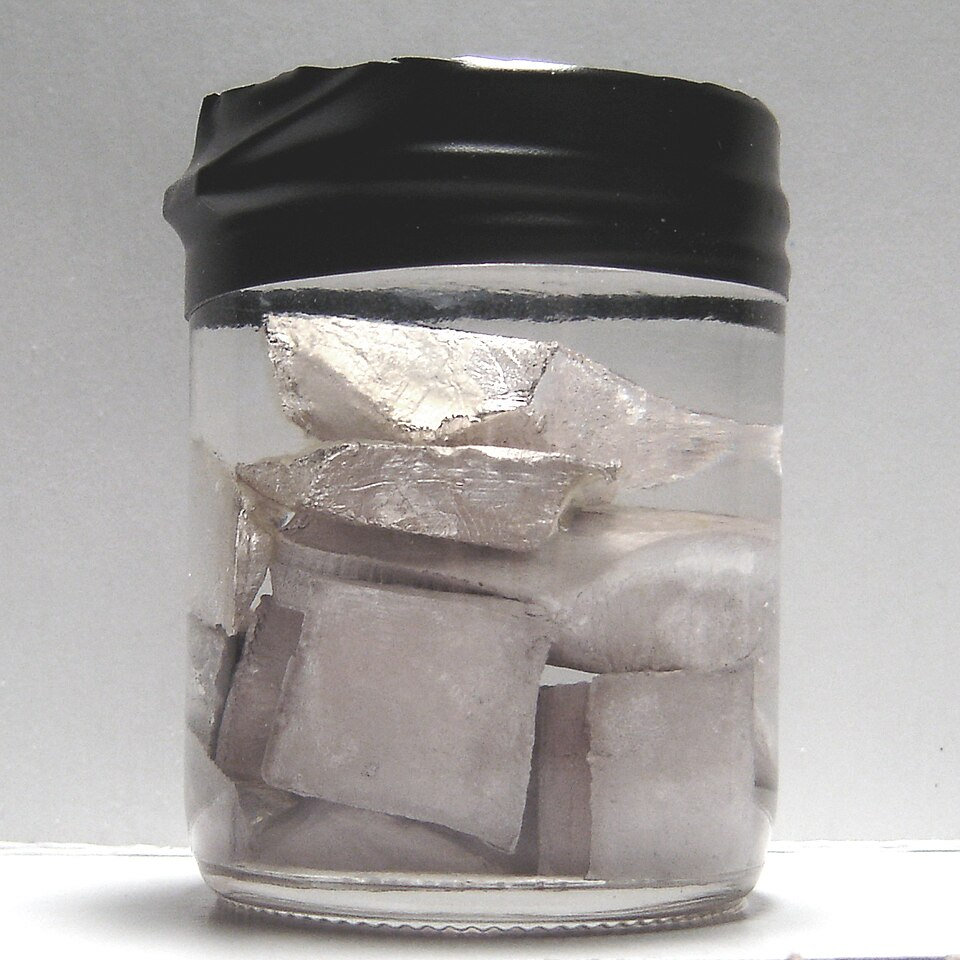
\includegraphics[height=4.6cm]{images/book2/sodium-oil.jpg}\hspace{0.8em}%
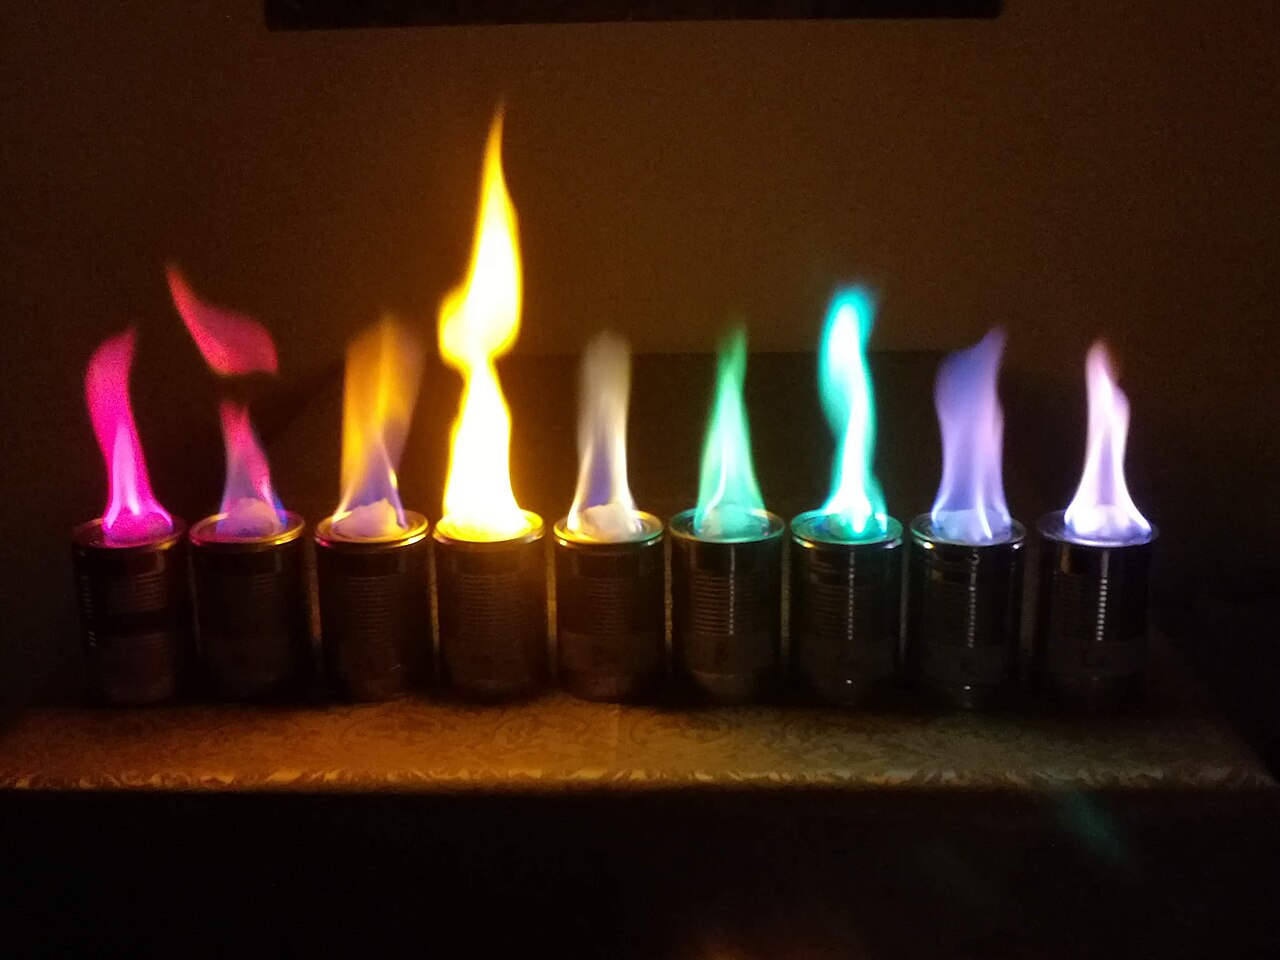
\includegraphics[height=4.6cm]{images/book2/flame-colours.jpg}

{\small يمينًا: يُحفظ الصوديوم تحت زيت معدني، بعيدًا عن الهواء والرطوبة
(صورة جاستن أورجيتيس، CC BY-SA 2.5). يسارًا: ألوان اللهب، من اليسار
إلى اليمين، لمركبات الليثيوم والسترونشيوم والكالسيوم والصوديوم والباريوم والبور والنحاس
والسيزيوم والبوتاسيوم: تعود الإلكترونات المثارة في اللهب إلى
مستويات أدنى فتصدر ضوءًا بأطوال موجية مميزة لكل عنصر
(\cref{ch:b1:quantum-numbers}) (صورة هيغلراست، CC BY-SA 4.0). كلتاهما من
ويكيميديا كومنز.}
\end{omfigure}

\begin{inthelab}[عرض، لا تجربة]
لا يُعرض تفاعل الصوديوم مع الماء إلا على يد المعلّم، خلف
حاجز أمان، بقطعة بحجم حبة العدس تُلقى في حوض كبير
من الماء يحتوي الفينولفثالين: فينصهر الفلز كرةً
راكضة، ويفور الهيدروجين، ويُظهر الأثر الوردي الهيدروكسيد
المتكوّن. أما البوتاسيوم فيشعل الهيدروجين. والقطع الأكبر تنفجر. ويُقطع الصوديوم
تحت الزيت، ويُمسك بالملقط، وتُهدم بقاياه بالإيثانول،
لا بالماء أبدًا.
\end{inthelab}

الليثيوم هو الاستثناء في زمرته: أصغر الأيونات، وأشدها
تميؤًا، ومن ثم أكثرها سالبيةً في الجهد، ومع ذلك أبطؤها
تفاعلًا مع الماء. وتشبه مركباته مركبات المغنيزيوم (فكربونات الليثيوم
وفوسفاته قليلة الذوبان، كما هي حال مركبات المغنيزيوم)، وهي
علاقة قطرية عبر الجدول الدوري. وتُنتج \omterm{def:b1:s-block:families}{الفلزات القلوية}
بالتحليل الكهربائي لكلوريداتها المنصهرة، إذ لا يوجد \omterm{def:b1:nernst:couple}{مختزل}
كيميائي قوي بما يكفي؛ وتفاعلات الأقطاب في مثل هذه الخلايا
تُدرس في مجلد السنة الثانية.

\section{مركبات الصوديوم في الصناعة}

\begin{definition}[طابع الأكاسيد]\label{def:b1:s-block:oxide-character}
\emph{الأكسيد القاعدي}\index{أكسيد قاعدي} يتفاعل مع الماء فيعطي
هيدروكسيدًا، أو مع الأحماض فيعطي أملاحًا (\ce{Na2O}، \ce{CaO})؛
و\emph{الأكسيد الحمضي}\index{أكسيد حمضي} يتفاعل مع الماء فيعطي حمضًا،
أو مع القواعد فيعطي أملاحًا (\ce{CO2}، \ce{SO3}، \ce{P4O10})؛
و\emph{الأكسيد المذبذب}\index{أكسيد مذبذب} يتفاعل مع الأحماض
والقواعد كلتيهما (\ce{Al2O3}، \ce{ZnO}). وعلى امتداد \omterm{def:b1:periodicity:table}{الدورة}، تنتقل الأكاسيد من قاعدية
(الفلزات، يسارًا) إلى حمضية (اللافلزات، يمينًا).
\end{definition}

يُصنع هيدروكسيد الصوديوم بالتحليل الكهربائي للمحلول الملحي (عملية
الكلور القلوي، التي تعطي أيضًا الكلور والهيدروجين). أما كربونات الصوديوم، أي رماد
الصودا، المستعملة في صناعة الزجاج والمنظفات واستخلاص الليثيوم، فإما تُستخرج من المناجم
على هيئة معدن الترونا وإما تُصنع من الملح والحجر الجيري: ففي سنة 2025
أنتج العالم نحو 71 مليون طن، منها 19 مليونًا من الرواسب الطبيعية و52
مليونًا مصنَّعة، معظمها بطريقة سولفاي.
% ledger: usgs:sodaash-total-2025, usgs:sodaash-natural-2025, usgs:sodaash-synthetic-2025

\begin{proposition}[طريقة سولفاي]\label{prop:b1:s-block:solvay}
تحوّل طريقة سولفاي كلوريد الصوديوم وكربونات الكالسيوم إلى
كربونات الصوديوم وكلوريد الكالسيوم، \ce{2NaCl + CaCO3 -> Na2CO3 +
CaCl2}، عبر خطوات تُعاد فيها الأمونيا وثنائي أكسيد الكربون إلى الدورة.
\end{proposition}

\begin{proof}
الخطوات هي: (1) \ce{CaCO3 -> CaO + CO2} (الفرن)؛ (2) \ce{NaCl + NH3 +
CO2 + H2O -> NaHCO3 + NH4Cl} (كربنة المحلول الملحي النشادري؛ ويترسب
الهيدروجين كربونات، وهو أقل الأملاح الموجودة ذوبانًا)؛ (3)
\ce{2NaHCO3 -> Na2CO3 + CO2 + H2O} (التكليس)؛ (4) \ce{CaO + H2O ->
Ca(OH)2}؛ (5) \ce{Ca(OH)2 + 2NH4Cl -> CaCl2 + 2NH3 + 2H2O} (استرجاع
الأمونيا). وبجمع $(1) + 2\times(2) + (3) + (4) + (5)$، تُختصر \ce{NH3}
و\ce{CO2} و\ce{NH4Cl} و\ce{NaHCO3} و\ce{CaO} و\ce{Ca(OH)2} والماء:
\ce{2NaCl + CaCO3 -> Na2CO3 + CaCl2}.
\end{proof}

\begin{omfigure}
\begin{tikzpicture}[font=\small, >={Stealth}, box/.style={draw, rounded corners, fill=omDef!8, minimum width=2.6cm, minimum height=0.8cm, align=center}]
  \node[box] (kiln) at (0,0) {فرن الجير\\\ce{CaCO3 -> CaO + CO2}};
  \node[box] (tower) at (5.3,0) {برج الكربنة\\\foreignlanguage{arabic}{يترسب \ce{NaHCO3}}};
  \node[box] (calc) at (10.2,0) {المكلِّس\\\ce{NaHCO3} $\to$ \ce{Na2CO3}};
  \node[box] (slake) at (0,-2.6) {مطفئ الجير\\\ce{CaO + H2O -> Ca(OH)2}};
  \node[box] (still) at (5.3,-2.6) {مقطّر الأمونيا\\\ce{NH4Cl + Ca(OH)2}};
  \draw[->, thick] (kiln) -- node[above] {\ce{CO2}} (tower);
  \draw[->, thick] (tower) -- node[above, font=\scriptsize] {\ce{NaHCO3}} (calc);
  \draw[->, thick] (calc.north) -- ++(0,0.6) -| node[pos=0.25, above] {\foreignlanguage{arabic}{\ce{CO2} المعاد تدويره}} (tower.north);
  \draw[->, thick] (kiln) -- node[left] {\ce{CaO}} (slake);
  \draw[->, thick] (slake) -- node[above, font=\scriptsize] {\ce{Ca(OH)2}} (still);
  \draw[->, thick] (tower) -- node[right] {\ce{NH4Cl}} (still);
  \draw[->, thick] (still.east) -- ++(1.2,0) |- node[pos=0.25, right] {\foreignlanguage{arabic}{\ce{NH3} المعاد تدويره}} ($(tower.east)+(0,-0.25)$);
  \draw[<-, thick] (tower.north west) -- ++(-0.5,0.6) node[above] {\foreignlanguage{arabic}{محلول ملحي \ce{NaCl}}};
  \draw[->, thick] (calc.east) -- ++(0.8,0) node[right] {\ce{Na2CO3}};
  \draw[->, thick] (still.south) -- ++(0,-0.6) node[below] {\ce{CaCl2}};
\end{tikzpicture}

{\small طريقة سولفاي. يدور ثنائي أكسيد الكربون والأمونيا في حلقات؛
ويدخل الملح والحجر الجيري، ويخرج رماد الصودا وكلوريد الكالسيوم.}
\end{omfigure}

\begin{omfigure}
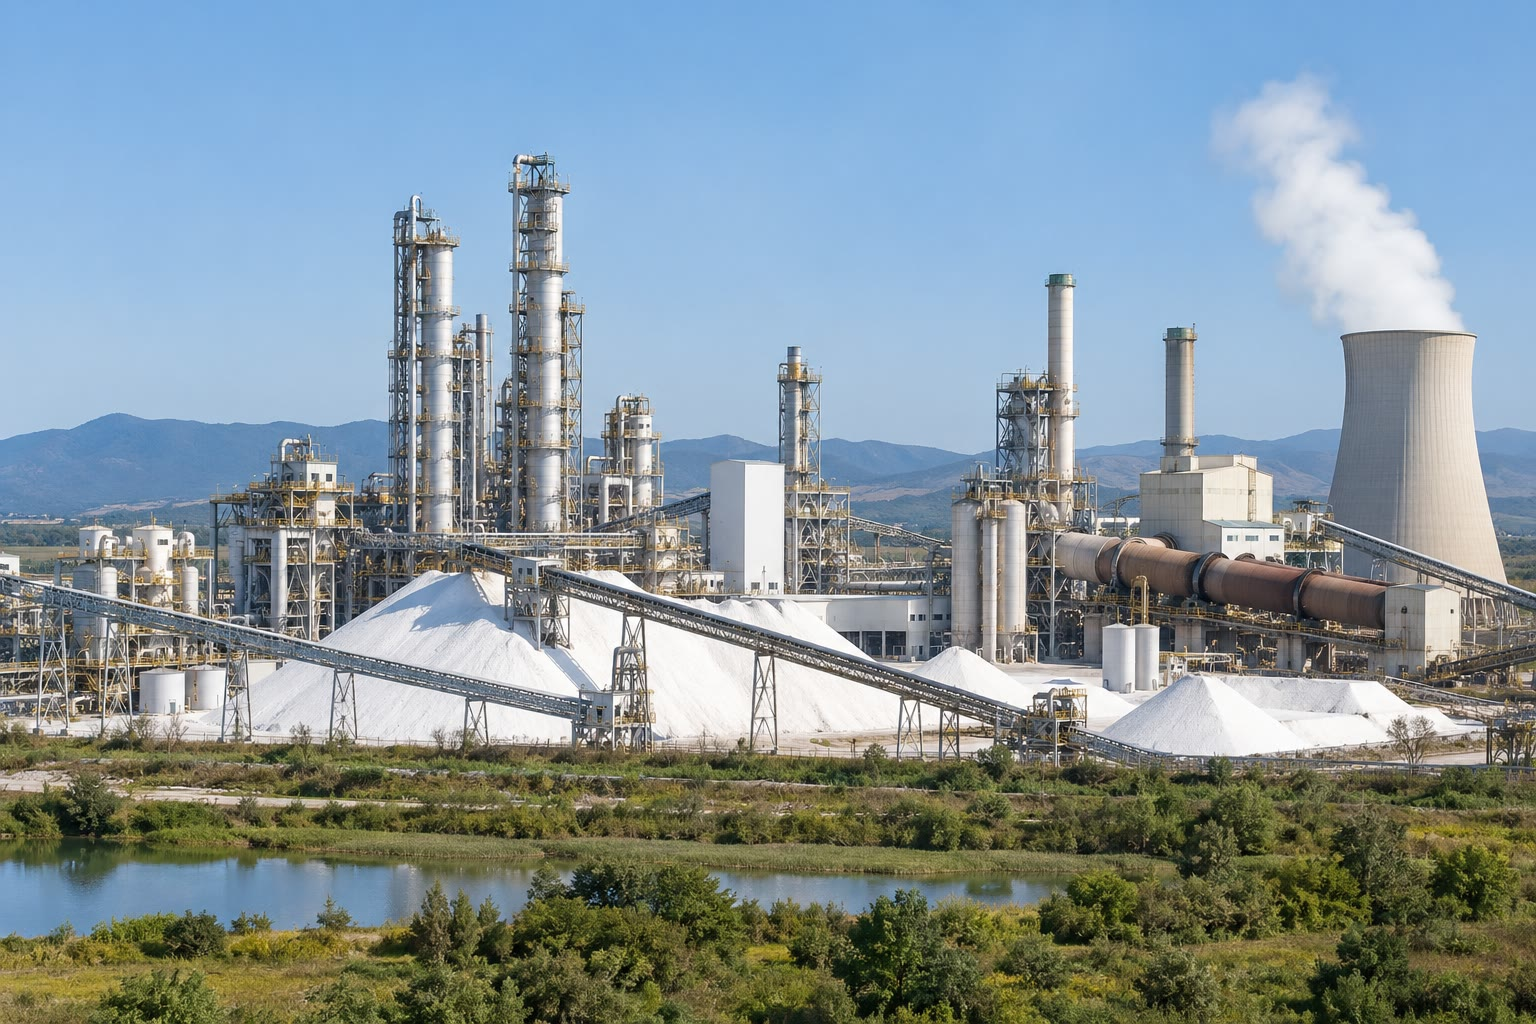
\includegraphics[width=0.55\linewidth]{images/book2/ai/b1-26-soda-ash-plant.jpg}

{\small مصنع لرماد الصودا: أفران الجير، وأبراج الكربنة، وأكوام من
كربونات الصوديوم.}
\end{omfigure}

\begin{method}[حصيلة الكتلة على مخطط التدفق]\label{met:b1:s-block:mass-balance}
\begin{enumerate}
  \item اكتب المعادلة الإجمالية (مجموع الخطوات، مع اختصار الأنواع
        المعاد تدويرها).
  \item احسب، انطلاقًا من الناتج المطلوب، كميات المواد الخام
        بالمعادلة الإجمالية، ثم صحّحها \omterm{def:b1:extent-q-and-k:fractional-extent}{بمردود} كل خطوة.
  \item ومن أجل نوع معاد تدويره، لا تحسب إلا كمية التعويض اللازمة لسد
        خسائره.
  \item تحقق من حصيلة كل عنصر بين المدخلات والمخرجات.
\end{enumerate}
\end{method}

\section{الفلزات القلوية الترابية}

المغنيزيوم والكالسيوم أقل نشاطًا من \omterm{def:b1:s-block:families}{الفلزات القلوية} (طاقات
تأينهما أعلى: Mg \qty{7.65}{eV}، Ca 6.11؛ وعليهما فقد إلكترونين) لكنهما
يبقيان مختزلين قويين ($E^\circ$ للمزدوجة $\ce{Mg^2+}/\ce{Mg}$ يساوي \babelsublr{$-2.36$~V}).
ويحترق المغنيزيوم في الهواء بضوء أبيض باهر؛ ويحميه غشاء أكسيده
عند درجة حرارة الغرفة. ويُسترجع المغنيزيوم من ماء البحر
بترسيب هيدروكسيده بالجير، $\mathrm{p}K_s = 11.25$
(\cref{ch:b1:precipitation}).
% ledger: ie:Mg, ie:Ca

\begin{proposition}[دورة الجير]\label{prop:b1:s-block:lime-cycle}
الحجر الجيري والجير الحي والجير المطفأ ثم الحجر الجيري من جديد تكوّن \omterm{def:b1:periodicity:table}{دورة}:
\ce{CaCO3 -> CaO + CO2} (بالتسخين في فرن)؛ \ce{CaO + H2O -> Ca(OH)2}
(الإطفاء، شديد الإطلاق للحرارة)؛ \ce{Ca(OH)2 + CO2 -> CaCO3 + H2O} (تصلّب
ملاط الجير في الهواء). والدورة بمجملها لا تغيّر شيئًا كيميائيًا،
لكنها تخزن الطاقة وثنائي أكسيد الكربون ثم تطلقهما.
\end{proposition}

\begin{proof}
بجمع المعادلات الثلاث، يُختصر كل نوع. وتفكك
الكربونات يتطلب حرارة، تنطلق من جديد في الخطوتين الأخريين؛
و\ce{CO2} المنطلق في الفرن يمتصه الملاط من جديد، ببطء.
\end{proof}

\begin{omfigure}
\begin{tikzpicture}[font=\small, >={Stealth}]
  \node[draw, rounded corners, fill=omDef!8] (a) at (90:2.0) {\foreignlanguage{arabic}{\ce{CaCO3} الحجر الجيري}};
  \node[draw, rounded corners, fill=omDef!8] (b) at (-30:2.0) {\foreignlanguage{arabic}{\ce{CaO} الجير الحي}};
  \node[draw, rounded corners, fill=omDef!8] (c) at (210:2.0) {\foreignlanguage{arabic}{\ce{Ca(OH)2} الجير المطفأ}};
  \draw[->, thick] (a) to[bend left=25] node[right, align=left] {حرارة\\$-\ce{CO2}$} (b);
  \draw[->, thick] (b) to[bend left=25] node[below] {$+\ce{H2O}$} (c);
  \draw[->, thick] (c) to[bend left=25] node[left, align=right] {$+\ce{CO2}$\\$-\ce{H2O}$} (a);
\end{tikzpicture}

{\small دورة الجير، من الحجر الجيري إلى الملاط ثم عودةً إلى كربونات
الكالسيوم.}
\end{omfigure}

\section{الليثيوم}

\begin{omfigure}
\begin{tikzpicture}
\begin{axis}[
  xbar, width=0.78\linewidth, height=5.4cm, xmin=0, xmax=110,
  symbolic y coords={CA,ML,BR,AR,ZW,CL,CN,AU}, ytick=data,
  yticklabels={كندا, مالي, البرازيل, الأرجنتين, زيمبابوي, تشيلي, الصين, أستراليا},
  xlabel={\foreignlanguage{arabic}{الليثيوم المستخرج سنة \babelsublr{2025}، تقديرات بآلاف الأطنان من \babelsublr{Li}}}, bar width=8pt,
  nodes near coords, every node near coord/.append style={font=\scriptsize},
  tick label style={font=\small}, label style={font=\small}, enlarge y limits=0.1]
\addplot[fill=omDef!45, draw=omDef] coordinates {(5.6,CA) (9.4,ML) (12,BR) (23,AR) (28,ZW) (56,CL) (62,CN) (92,AU)};
\end{axis}
\end{tikzpicture}

{\small أكبر منتجي الليثيوم سنة 2025 (تقديرات؛ والمجموع العالمي
نحو \num{290000} طن من الليثيوم). تستخرج أستراليا الصخور الصلبة
(السبودومين)؛ وتضخ تشيلي والأرجنتين المحاليل الملحية.}
% ledger: usgs:li-canada-2025, usgs:li-mali-2025, usgs:li-brazil-2025, usgs:li-argentina-2025, usgs:li-zimbabwe-2025, usgs:li-chile-2025, usgs:li-china-2025, usgs:li-australia-2025, usgs:li-world-2025
\end{omfigure}

يُركَّز المحلول الملحي بالتبخير، ويُزال المغنيزيوم بالجير، ثم
تُرسَّب كربونات الليثيوم برماد الصودا. ولكربونات الليثيوم
خاصية غير مألوفة: فذوبانيتها على الساخن أقل منها على البارد: \qty{1.31}{\percent}
كتليًا عند \qty{20}{\celsius}، و\qty{0.84}{\percent} عند \qty{80}{\celsius}،
و\qty{0.71}{\percent} عند \qty{100}{\celsius}. ولذلك تُرسَّب
من محلول ساخن، كما تحسب مسألة نهاية الأسبوع.
% ledger: sol:Li2CO3-20, sol:Li2CO3-80, sol:Li2CO3-100

\section{تمارين}

\begin{exercise}[$\star$]\label{exo:b1:s-block:1}
صنّف إلى \omterm{def:b1:s-block:hydride}{هيدريد ملحي} أو تساهمي أو فلزي: \ce{KH}، \ce{SiH4}،
\ce{CaH2}، \ce{H2S}، \ce{PdH_{0.6}}. واكتب تفاعل \ce{CaH2} مع الماء.
\end{exercise}

\begin{exercise}[$\star$]\label{exo:b1:s-block:2}
اكتب تفاعلات الليثيوم والصوديوم والبوتاسيوم مع الماء، وتفاعل
المغنيزيوم مع حمض الهيدروكلوريك المخفف.
\end{exercise}

\begin{exercise}[$\star$]\label{exo:b1:s-block:3}
صنّف إلى قاعدي أو حمضي أو مذبذب: \ce{Na2O}، \ce{MgO}، \ce{Al2O3}،
\ce{SiO2}، \ce{SO3}، \ce{ZnO}، \ce{CO2}. واكتب تفاعلًا واحدًا لكل نوع.
\end{exercise}

\begin{exercise}[$\star$]\label{exo:b1:s-block:4}
احسب ثابت التفاعل \ce{2Na + 2H2O -> 2Na+ + 2OH- + H2} عند pH يساوي 14 انطلاقًا من
\omterm{def:b1:nernst:electrode-potential}{الجهود المعيارية}.
\end{exercise}

\begin{exercise}[$\star\star$]\label{exo:b1:s-block:5}
فسّر ألوان لهب الليثيوم (أحمر) والصوديوم (أصفر) مستعملًا
\omterm{def:b1:quantum-numbers:energy-level}{مستويات طاقة} الذرات (\cref{ch:b1:quantum-numbers}). وما طاقة
فوتون أصفر طول موجته \qty{589}{nm}؟
\end{exercise}

\begin{exercise}[$\star\star$]\label{exo:b1:s-block:6}
احسب كتلة الحجر الجيري (\ce{CaCO3} النقي) وكتلة كلوريد الصوديوم
اللازمتين لطن واحد من رماد الصودا بطريقة سولفاي، \omterm{def:b1:extent-q-and-k:fractional-extent}{بمردود} إجمالي
قدره \qty{90}{\percent} بالنسبة إلى كلوريد الصوديوم.
\end{exercise}

\begin{exercise}[$\star\star$]\label{exo:b1:s-block:7}
يحتوي ماء البحر نحو \qty{1.3}{g/L} من المغنيزيوم (معطيات
التمرين). عند أي pH يبدأ هيدروكسيد المغنيزيوم بالترسب؟
وما كتلة الجير المطفأ التي ترسّب مغنيزيوم \qty{1.0}{m^3}؟
\end{exercise}

\begin{exercise}[$\star\star$]\label{exo:b1:s-block:8}
لماذا يتفاعل الليثيوم مع الماء أبطأ من البوتاسيوم، مع أن
جهده المعياري أدنى؟ ميّز بين الديناميكا الحرارية والحركية.
\end{exercise}

\begin{exercise}[$\star\star$]\label{exo:b1:s-block:9}
احسب كتلة الجير الحي المحصَّل عليها من طن واحد من الحجر الجيري
وحجم \ce{CO2} المنطلق، عند \qty{25}{\celsius} و\qty{1}{bar}.
\end{exercise}

\begin{exercise}[$\star\star\star$]\label{exo:b1:s-block:10}
استخرج العالم نحو \num{290000} طن من الليثيوم سنة 2025. فما كتلة
كربونات الليثيوم الموافقة؟ وإذا كانت بطارية سيارة تحتوي \qty{8}{kg} من
الليثيوم (معطيات التمرين)، فكم بطارية يمكن أن يزوّد بها؟
\end{exercise}

\begin{exercise}[$\star\star\star$]\label{exo:b1:s-block:11}
بيّن انطلاقًا من معطيات الفصل أن \omterm{def:b1:precipitation:solubility}{ذوبانية} كربونات الليثيوم تنخفض مع درجة الحرارة،
وفسّر لماذا يحسّن ترسيبها على الساخن
استرجاعها من المحلول الملحي.
\end{exercise}

\begin{exercise}[$\star\star\star$]\label{exo:b1:s-block:12}
في الخطوة (2) من طريقة سولفاي، يحتوي المحلول على \ce{Na+}،
و\ce{NH4+}، و\ce{Cl-} و\ce{HCO3-}. فسّر لماذا يترسب هيدروجين كربونات الصوديوم
بدل كلوريد الأمونيوم، ولماذا تحتاج الطريقة إلى
الأمونيا لا إلى هيدروكسيد الصوديوم.
\end{exercise}

\section{مسألة: الليثيوم من المحلول الملحي}

\begin{problem}[{مسألة نهاية الأسبوع --- تركيز محلول ملحي ليثيومي،
وإزالة المغنيزيوم بالجير، وترسيب كربونات الليثيوم برماد
الصودا، وكتلة كربونات الليثيوم المسترجعة من متر مكعب واحد}]
\label{pb:b1:s-block:1}
يحتوي محلول ملحي مضخوخ من تحت سبخة ملحية \qty{1.5}{g/L} من الليثيوم
و\qty{0.60}{g/L} من المغنيزيوم (على هيئة أيونات، مع كثير من كلوريد الصوديوم).
ويركّزه التبخير في الأحواض أربع مرات. ثم يُعالج متر مكعب واحد من
المحلول الملحي المركّز: يزيل الجير المغنيزيوم، ويزيل رماد الصودا
الكالسيوم، ثم يرسّب رماد الصودا الساخن أخيرًا كربونات الليثيوم عند
\qty{80}{\celsius}. المعطيات: الكتل المولية (\unit{g/mol}) Li 6.9، Mg 24.3،
\ce{Ca(OH)2} 74.1، \ce{Na2CO3} 106.0، \ce{Li2CO3} 73.8؛ $\mathrm{p}K_s$
\ce{Mg(OH)2} 11.25، \ce{CaCO3} 8.30؛ $\mathrm{p}K_e = 14.00$؛ \omterm{def:b1:precipitation:solubility}{ذوبانية}
\ce{Li2CO3} \qty{0.84}{\percent} كتليًا عند \qty{80}{\celsius}؛ واعتبر
السائل النهائي \qty{1.00}{m^3} كثافته \qty{1.0}{kg/L}.

\medskip
\noindent\textbf{الجزء الأول --- التركيز.}
\begin{enumerate}
  \item احسب تركيزي الليثيوم والمغنيزيوم في المحلول الملحي
        المركّز.
  \item ما حجم الماء الذي يتبخر لكل متر مكعب من المحلول الملحي
        المركّز؟
  \item لماذا يُستعمل التبخير الشمسي لا التسخين؟
  \item أي ملح يتبلور أولًا في الأحواض، ولماذا؟
  \item احسب كميتي الليثيوم والمغنيزيوم في متر مكعب واحد.
  \item لماذا يجب إزالة المغنيزيوم قبل ترسيب الليثيوم؟
\end{enumerate}

\medskip
\noindent\textbf{الجزء الثاني --- إزالة المغنيزيوم والكالسيوم.}
\begin{enumerate}[resume]
  \item اكتب تفاعل أيونات المغنيزيوم مع الجير المطفأ.
  \item احسب كتلة الجير المطفأ اللازمة (بالنسب التكافئية).
  \item عند أي pH يترسب \qty{99.9}{\percent} من المغنيزيوم؟
  \item لماذا لا يترسب الليثيوم على هيئة هيدروكسيده؟
  \item اكتب إزالة الكالسيوم المُدخَل، برماد الصودا.
  \item احسب كتلة رماد الصودا اللازمة لتلك الخطوة.
\end{enumerate}

\medskip
\noindent\textbf{الجزء الثالث --- كربونات الليثيوم.}
\begin{enumerate}[resume]
  \item اكتب ترسيب كربونات الليثيوم.
  \item احسب كتلة رماد الصودا اللازمة لليثيوم.
  \item احسب الكتلة النظرية لكربونات الليثيوم.
  \item لماذا يُجرى الترسيب عند \qty{80}{\celsius}؟
  \item ما كتلة كربونات الليثيوم التي تبقى ذائبة في السائل؟
  \item كيف يُغسل الراسب دون فقد كثير منه؟
\end{enumerate}

\medskip
\noindent\textbf{الجزء الرابع --- الحصيلة.}
\begin{enumerate}[resume]
  \item احسب كتلة كربونات الليثيوم المسترجعة.
  \item احسب نسبة استرجاع الليثيوم.
  \item اقترح ما يُفعل بالسائل.
  \item قارن الليثيوم في متر مكعب واحد بالإنتاج العالمي
        سنة 2025: كم مترًا مكعبًا يمثّل ذلك الإنتاج؟
  \item اذكر كتلة كربونات الليثيوم المسترجعة لكل متر مكعب من المحلول
        الملحي المركّز.
\end{enumerate}
\end{problem}
